\documentclass[12pt,a4paper]{article}

% Paquetes esenciales
\usepackage[utf8]{inputenc}
\usepackage[spanish,es-tabla]{babel}
\usepackage[margin=2.54cm]{geometry}
\usepackage{graphicx}
\usepackage{float}
\usepackage{booktabs} 
\usepackage{csquotes} 
\usepackage{xcolor}
\usepackage[hidelinks]{hyperref}

% Configuración de referencias IEEE con biblatex
\usepackage[backend=biber, style=ieee]{biblatex}
\addbibresource{referencias.bib}

\begin{document}

\begin{titlepage}
    \centering
    \vspace*{2cm}
    
    {\Large \textbf{Universidad Técnica Estatal de Quevedo (UTEQ)}}\\[0.5cm]
    {\large Facultad de Ciencias de la Ingeniería}\\[0.5cm]
    {\large Carrera de Ingeniería de Software}\\[2cm]
    
    {\large \textbf{Asignatura:} Sistemas Distribuidos}\\[0.5cm]
    {\large \textbf{Código de la Actividad:} TA-IND-01}\\[1.5cm]
    
    {\Large \textbf{Análisis crítico de InfluxDB y comparación arquitectónica con Prometheus}}\\[2cm]
    
    {\large \textbf{Estudiante:} Cesar Abrahan Macias Vasquez}\\[0.5cm]
    {\large \textbf{Paralelo:} 7mo B}\\[0.5cm]
    {\large \textbf{Fecha:} 15 de noviembre de 2026}\\[1cm]
    
    {\large \textbf{URL del Repositorio:} \url{https://github.com/CesarMacias007/TA-IND-01-Informe-Acad-mico-Individual-An-lisis-Cr-tico-de-Sistemas-Distribuidos.git}}
    
    \vfill
\end{titlepage}

\begin{abstract}
Este informe presenta un análisis crítico de la arquitectura distribuida de InfluxDB, una base de datos especializada en series temporales (TSDB), contrastándola con el modelo operativo de Prometheus. A través de los conceptos fundamentales de sistemas distribuidos, se evalúa cómo InfluxDB implementa las transparencias de ubicación y replicación mediante su API unificada, y cómo resuelve las disyuntivas del teorema CAP priorizando la consistencia (CP) en su metadata mediante el algoritmo Raft, pero favoreciendo la disponibilidad (AP) en la ingesta de datos a través de mecanismos como \textit{Hinted Handoff}. El estudio detalla las implicaciones del modelo de comunicación asincrónico \textit{Push} frente al \textit{Pull}, la tolerancia a fallos ante eventos reales como la degradación por explosión de cardinalidad, y presenta un escenario de experimentación propia mediante despliegue en contenedores. Finalmente, se argumentan las fortalezas y limitaciones del sistema, contextualizando sus compromisos arquitectónicos con ejemplos del entorno cotidiano local e informático.
\end{abstract}

\section{Introducción}
El auge de la Internet de las Cosas (IoT) y la monitorización de infraestructura ha impulsado la necesidad de sistemas distribuidos capaces de ingerir y consultar volúmenes masivos de datos temporales con baja latencia \cite{kopp2025}. InfluxDB se presenta como una base de datos de series temporales (TSDB) de alto rendimiento diseñada específicamente para este propósito \cite{bader2021}. A diferencia de las bases de datos relacionales o de documentos tradicionales, InfluxDB optimiza el almacenamiento continuo de métricas estructuradas en el tiempo, siendo ampliamente utilizada en entornos de observabilidad a gran escala \cite{tripathi2023}. 

Se eligió analizar InfluxDB debido a su arquitectura distribuida híbrida, la cual resuelve los desafíos de particionamiento de red y consistencia de manera distinta a otros sistemas del mercado, como Prometheus. El objetivo de este informe es evaluar críticamente cómo InfluxDB implementa las transparencias de distribución, su comportamiento frente al teorema CAP y su modelo de comunicación orientado a eventos.

\section{Arquitectura del Sistema}
La arquitectura distribuida de InfluxDB (en su versión Enterprise o clúster) separa lógicamente el procesamiento de ingesta, el almacenamiento de datos y la gestión de metadatos para lograr escalabilidad horizontal \cite{ford2021}. Sus componentes principales son:

\begin{itemize}
    \item \textbf{API HTTP (Ingesta y Consulta):} Actúa como la puerta de enlace para los clientes, recibiendo datos a través de peticiones asincrónicas en un formato optimizado llamado \textit{Line Protocol}.
    \item \textbf{Nodos de Datos (Data Nodes):} Responsables del almacenamiento físico de las series temporales. Utilizan un motor de almacenamiento propio llamado TSM (\textit{Time-Structured Merge Tree}) respaldado por un WAL (\textit{Write-Ahead Log}) para garantizar la durabilidad \cite{silva2023}.
    \item \textbf{Nodos Meta (Meta Nodes):} Mantienen el estado global del clúster, gestionando la topología, la ubicación de los \textit{shards} (fragmentos de datos) y la autenticación. 
\end{itemize}

Ambos tipos de nodos se comunican de forma asincrónica, permitiendo que el sistema mantenga la ingesta de datos incluso si algunos nodos de almacenamiento presentan latencia o fallos temporales.

\begin{figure}[H]
    \centering
    % 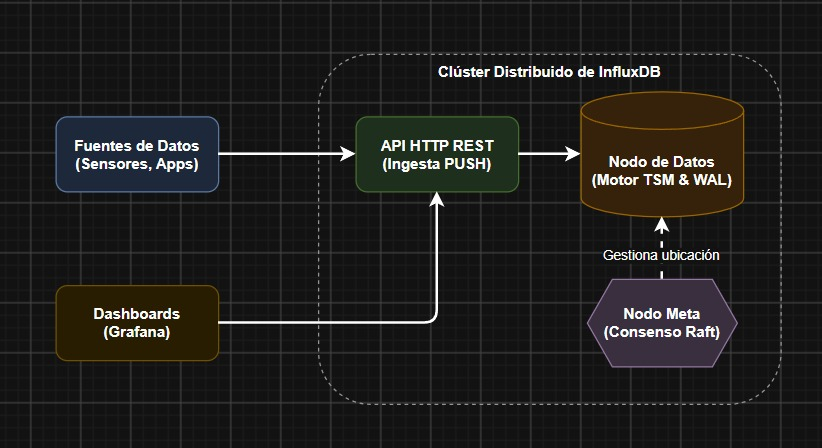
\includegraphics[width=0.8\textwidth]{arquitectura.jpeg}
    \caption{Arquitectura distribuida de InfluxDB.}
    \label{fig:arquitectura}
\end{figure}

\section{Análisis con los Conceptos de la Unidad 1}

\subsection{Transparencias de Distribución}
InfluxDB logra abstraer la complejidad de su clúster para los desarrolladores a través de múltiples transparencias de distribución:
\begin{itemize}
    \item \textbf{Transparencia de Ubicación y Acceso:} Los clientes interactúan exclusivamente con una única API HTTP RESTful. El usuario envía una métrica sin necesidad de conocer en qué nodo físico o \textit{shard} del clúster se almacenará finalmente el dato.
    \item \textbf{Transparencia de Replicación:} El sistema permite configurar un factor de replicación (ej. $N=3$). El usuario escribe el dato una sola vez, y el sistema se encarga de propagarlo a los nodos correspondientes de forma invisible \cite{silva2023}.
    \item \textbf{Transparencia de Fallos (Parcial):} Si un nodo de datos cae, las consultas se enrutan automáticamente a las réplicas disponibles. Sin embargo, no es completamente transparente en escenarios de consistencia estricta, ya que las lecturas pueden retornar datos desactualizados (consistencia eventual).
\end{itemize}

\subsection{Teorema CAP y PACELC}
InfluxDB adopta un enfoque híbrido frente al teorema CAP, separando el tratamiento de los metadatos y los datos de series temporales \cite{tripathi2023}:
\begin{itemize}
    \item \textbf{Metadatos (CP - Consistencia y Tolerancia a Particiones):} Para la gestión de la topología del clúster, los Nodos Meta utilizan el algoritmo de consenso Raft. Ante una partición de red, si no hay un cuórum mayoritario, el clúster rechaza cambios en su estructura para mantener la consistencia estricta \cite{blinowski2022}.
    \item \textbf{Datos (AP - Disponibilidad y Tolerancia a Particiones):} Para la ingesta de métricas, InfluxDB prioriza la disponibilidad. Si un nodo de datos destino está inaccesible debido a una partición, el nodo receptor almacena temporalmente los datos en una cola llamada \textit{Hinted Handoff}. Una vez que el nodo caído se recupera, los datos se sincronizan.
\end{itemize}
Bajo la extensión PACELC, en ausencia de particiones (E), el sistema prioriza la latencia (L) sobre la consistencia (C), respondiendo a los clientes tan pronto como el dato es escrito en la memoria y en el WAL, antes de que se replique por completo.

\subsection{Modelos de Comunicación}
A diferencia de los sistemas de monitorización basados en el modelo \textit{Pull} (donde el servidor interroga periódicamente a los clientes), InfluxDB implementa un modelo \textit{Push}. Los agentes emisores inician la comunicación enviando datos activamente hacia la API HTTP mediante peticiones \texttt{POST}. Este enfoque asincrónico por lotes (\textit{batching}) reduce la sobrecarga de conexiones persistentes y aísla al clúster, ya que este no necesita conocer previamente las direcciones IP o la topología de los dispositivos IoT que le reportan \cite{bader2021}.

\subsection{Tolerancia a Fallos e Incidentes en Producción}
El diseño de InfluxDB absorbe fallos transitorios utilizando el mecanismo de \textit{Hinted Handoff} previamente descrito. Las caídas abruptas de energía se mitigan con el registro continuo en el WAL (\textit{Write-Ahead Log}), lo que permite al motor TSM reconstruir el estado en memoria al reiniciar.

No obstante, el sistema presenta vulnerabilidades documentadas frente al agotamiento de recursos. Dado que InfluxDB prioriza aceptar el tráfico de ingesta continuo por sobre las tareas internas de compactación de disco, un incidente recurrente en instancias masivas es la terminación abrupta por falta de memoria (OOM - \textit{Out Of Memory}) %
 derivado de una explosión de cardinalidad (indexar erróneamente valores infinitos como UUIDs en las etiquetas) \cite{githubOOM}. %
 Asimismo, ocurren bloqueos a gran escala, como el incidente documentado en septiembre de 2026 en InfluxDB Cloud (región Azure West Europe), donde una prolongada degradación de consultas provocó tiempos de espera críticos, obligando a duplicar la memoria base para el \textit{page cache} y el rendimiento de disco de los nodos para estabilizar la plataforma \cite{pulsapi2026}. %

\section{Experimentación Propia}
Para evidenciar empíricamente los límites de disponibilidad ante particiones (AP del teorema CAP) en sistemas de nodo único y comprobar el modelo \textit{Push}, se desplegó InfluxDB 1.8 en contenedores Docker mediante GitHub Codespaces (ver Anexo B). 

Durante la prueba, se simuló a un cliente enviando métricas asincrónicas de temperatura mediante \texttt{cURL} hacia la API HTTP. Posteriormente, se forzó la caída del clúster deteniendo el contenedor. Al intentar enviar una nueva métrica durante la interrupción, el servidor retornó inmediatamente un rechazo de red (\textit{Connection refused}). Esto corroboró que, al carecer de una capa de réplicas que gestione el \textit{Hinted Handoff}, la responsabilidad de encolar y reintentar el envío recae completamente sobre el agente productor.

\section{Ejemplos del Entorno del Estudiante}
Las disyuntivas arquitectónicas de los sistemas distribuidos son perceptibles en aplicaciones cotidianas:
\begin{itemize}
    \item \textbf{SGA de la UTEQ (Disponibilidad frente a Consistencia):} Durante la temporada masiva de matriculación, la infraestructura prioriza mantenerse en línea para despachar las páginas web (Disponibilidad). Esto genera un modelo de consistencia eventual; un estudiante puede visualizar un paralelo con cupos disponibles en su caché local y, segundos después, al intentar registrarse, el servidor rechaza la transacción porque el estado central ya cambió.
    \item \textbf{Multijugador GTA Online (Modelos Híbridos):} El juego aplica dos estrategias de red distintas. Para el movimiento en el mundo abierto, utiliza sincronización casi \textit{Peer-to-Peer} (P2P), minimizando la latencia. Sin embargo, para eventos críticos, como alterar el dinero en la cuenta bancaria del personaje, cambia a un modelo Cliente-Servidor estricto, priorizando la consistencia fuerte para evitar transacciones no autorizadas.
\end{itemize}

\section{Análisis Comparativo: InfluxDB vs Prometheus}
\begin{table}[H]
    \centering
    \caption{Comparativa arquitectónica de Bases de Datos de Series Temporales}
    \begin{tabular}{@{}p{3.5cm} p{5.5cm} p{5.5cm}@{}}
        \toprule
        \textbf{Criterio (Unidad 1)} & \textbf{InfluxDB} & \textbf{Prometheus} \\ \midrule
        \textbf{Comunicación} & Push (HTTP POST activo) & Pull (Scraping periódico HTTP GET) \\
        \textbf{Teorema CAP} & Prioriza AP (Hinted Handoff) & Prioriza CP local / Alta Disponibilidad vía pares \\
        \textbf{Ubicación}& Transparencia alta (API única)& Transparencia baja (Requiere Service Discovery)\\
        \textbf{Redundancia} & Nativa (Raft y fragmentación) & Réplicas independientes sin clúster nativo \\
        \textbf{Casos Ideales} & Eventos irregulares (IoT) y logs & Topologías dinámicas efímeras (Kubernetes) \\
        \bottomrule
    \end{tabular}
\end{table}

La disparidad principal radica en la iniciativa de la comunicación. Prometheus domina ecosistemas de microservicios nativos de la nube porque su modelo \textit{Pull} descubre dinámicamente si un contenedor muere, dejando de recolectar basura automáticamente. Por el contrario, InfluxDB es estructuralmente superior cuando se requiere registrar latencias de eventos impredecibles y cuando los clientes de origen (como sensores en fincas) se encuentran detrás de firewalls y NAT estáticos, obligando al sistema a recibir datos (\textit{Push}) en lugar de ir a buscarlos.

\section{Postura Crítica}
La especialización del motor TSM de InfluxDB permite ingerir cientos de miles de eventos por segundo, pero su arquitectura introduce compromisos severos. Al depender del cliente para iniciar el modelo \textit{Push}, InfluxDB es vulnerable a ataques de denegación por flujo descontrolado, requiriendo robustas colas externas (como Kafka) en entornos masivos. Adicionalmente, el ecosistema penaliza dramáticamente el mal diseño de esquemas: si un desarrollador indexa datos infinitos en las etiquetas (como hashes de sesión), se genera una sobrecarga térmica en la memoria del sistema operativo. Por tanto, en arquitecturas donde los datos requieren vínculos relacionales fuertes o estricto cumplimiento ACID para transacciones comerciales, bases tradicionales distribuidas como CockroachDB serían una opción operativa mucho más estable.

\section{Conclusiones}
\begin{itemize}
    \item La separación algorítmica entre la gestión del clúster mediante Raft (CP) y el almacenamiento físico (AP) permite a InfluxDB soportar ráfagas agresivas de ingesta sin corromper la consistencia de su topología.
    \item La experimentación en un entorno aislado ratificó que el modelo \textit{Push} por HTTP facilita la escalabilidad y transparencia de acceso a costa de delegar la recuperación de fallas de red al productor del dato.
    \item Todos los sistemas distribuidos evaluados exigen ceder consistencia inmediata para ganar tolerancia a las particiones de red (PACELC), un sacrificio perfectamente asimilable en métricas de observabilidad.
\end{itemize}

\section{Declaración de Uso de Inteligencia Artificial}
Para la elaboración de este informe se utilizó la inteligencia artificial Gemini como herramienta de apoyo en la estructuración de sintaxis LaTeX, integración bibliográfica y en el mapeo de detalles técnicos sobre incidentes comprobables. El diseño lógico de la arquitectura, el análisis comparativo, el proceso de experimentación en contenedores y el razonamiento conceptual frente a los sistemas del entorno cotidiano fueron analizados, validados y concluidos de manera totalmente autónoma.

\newpage
\appendix
\section{Anexo A: Evolución de la Arquitectura}
\begin{figure}[H]
    \centering
    % Descomenta y asegúrate de tener la imagen subida
    % 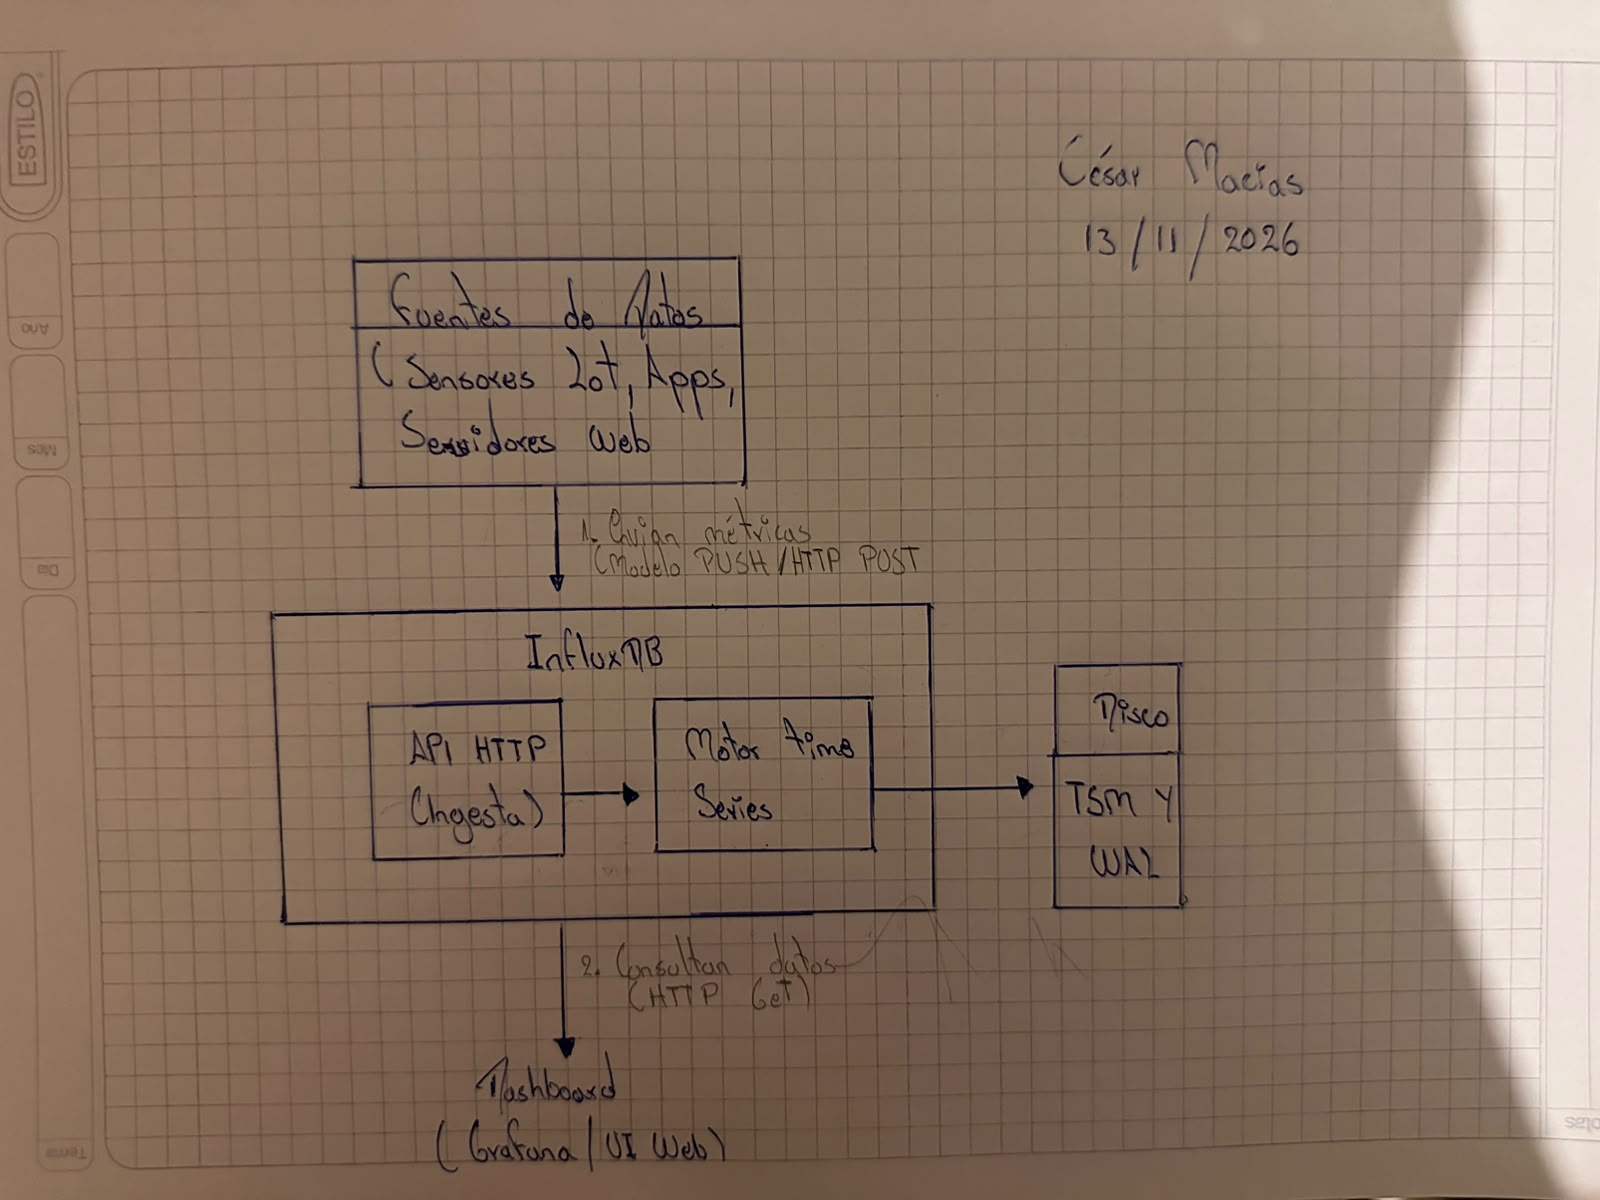
\includegraphics[width=0.7\textwidth]{esquema.jpeg}
    \caption{Bosquejo inicial a mano de los componentes del sistema.}
\end{figure}

\section{Anexo B: Evidencia de Lectura de Fuentes y Experimentación}
\begin{figure}[H]
    \centering
    % \includegraphics[width=0.7\textwidth]{capturas_fuentes_1.jpg}
    \caption{Evidencia fotográfica del proceso de documentación técnica e interacción local con la base de datos.}
\end{figure}

\printbibliography[heading=bibintoc, title={Referencias}]
\end{document}
